\subsection{Ejemplos de \frameworksPC \ecommerceCOM existentes}

He aquí hay una lista de 11 soluciones \ecommerceCOM \openSourcePC. El \coreAS de todas las aplicaciones es \freePC. Cada aplicación tiene extensiones \freePC y \premium, y opciones de soporte para mejorar el desarrollo de la \store.

\begin{itemize}
	\item \textbf{\nameOpenCart}. Es una aplicación \openSourcePC, basada en \phpNAME, es una solución \ecommerceCOM para comerciantes \online. \nameOpenCart tiene una comunidad activa y leal para el apoyo de usuarios, así como una lista de socios comerciales para instalación y customización profesional. En \nameOpenCart existen más de 20 medios de pago y más de 8 métodos de envío para la descarga por defecto, con cientos de métodos adicionales para el envío y el pago en su directorio de extensiones. \nameOpenCart también fue diseñado para un manejo sencillo de múltiples compras desde una interfaz de administración. Tiene más de 2700 \themesCPT.
	
	\begin{figure}[H]
		\centering
		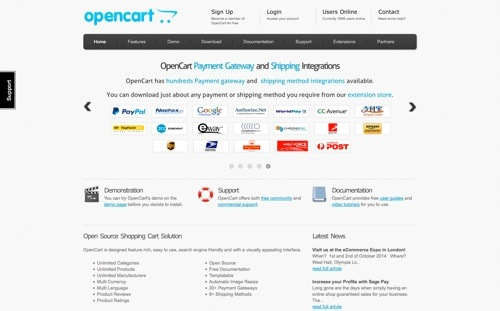
\includegraphics[width=0.5\textwidth]{figuras/cap1/openCartWebsite.jpg}
		\caption{\nameOpenCart \websiteINT \cite{online_OpenCartWebsite}.}
	\end{figure}


	\item \textbf{\namePrestaShop}. Es una solución \ecommerceCOM \openSourcePC, escrita en \phpNAME y basada en \smartyTemplateEngine. \namePrestaShop viene con más de 310 características integradas y 3500 módulos y \templatesAS. Cuenta con ventas cruzadas, productos descargables, la exportación de productos, una pagina de pago, envío, descuentos y mucho más. Descargado más de 4 millones de veces, \namePrestaShop es usado en 160 países y traducido a 63 idiomas. Tiene más de 600000 miembros en su comunidad.

	\begin{figure}[H]
		\centering
		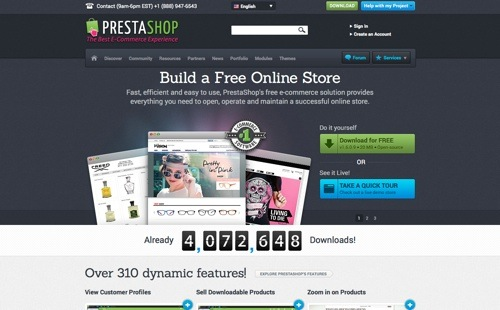
\includegraphics[width=0.5\textwidth]{figuras/cap1/PrestaShopWebsite.jpg}
		\caption{\namePrestaShop \websiteINT \cite{online_PrestaShop}.}
	\end{figure}


	\item \textbf{\nameMagento \Community \Edition} es una versión \freePC y \openSourcePC de una plataforma \ecommerceCOM. Los comerciantes pueden acceder a características adicionales instalando las extensiones desde el gran \nameMagento \connectCustom \marketplace. No existe soporte para \nameMagento \Community \Edition, así que las respuestas a las preguntas técnicas deben ser resueltas a través del foro de usuarios. Un detalle, \nameMagento ha anunciado el cierro de su \hosted \solution, \nameMagento \go, por ahora no habría problemas con \Community \Edition. \nameMagento \Community \Edition soporta más de 200000 sitios de clientes.

	\begin{figure}[H]
		\centering
		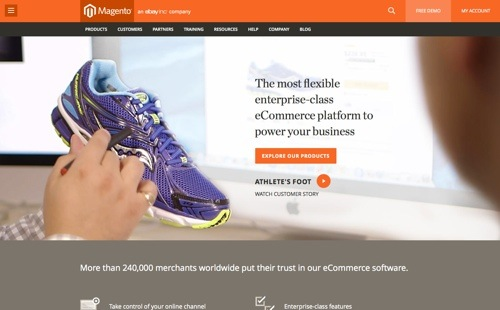
\includegraphics[width=0.5\textwidth]{figuras/cap1/MagentoWebsite.jpg}
		\caption{\nameMagento \websiteINT \cite{online_Magento}.}
	\end{figure}


	\item \textbf{\nameZenCart} es una aplicación \ecommerceCOM \openSourcePC escrita en \phpNAME.\nameZenCart \branched desde el código \nameOsCommerce en 2003, con una solución que era más \templateBased. Tiene más de 1800 \addOns en 16 categorías. La comunidad de apoyo de \nameZenCart tiene aproximadamente 150000 miembros y 200000 \threadsPL.

	\begin{figure}[H]
		\centering
		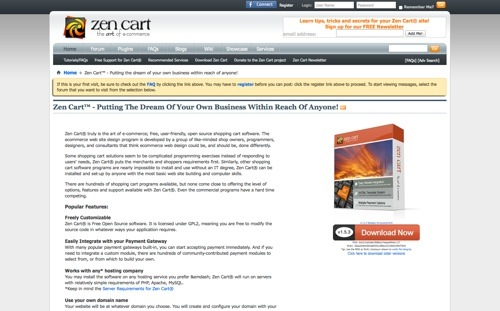
\includegraphics[width=0.5\textwidth]{figuras/cap1/ZenCartWebsite.jpg}
		\caption{\nameZenCart \websiteINT \cite{online_ZenCart}.}
	\end{figure}


	\item \textbf{\nameSpreeCommerce} es una solución \ecommerceCOM \openSourcePC  basado en \rubyonrailsNAME. La plataforma modular permite configurar, complementar, o reemplazar cualquier funcionalidad que necesites. \nameSpreeCommerce tiene más de 45000 tiendas; la plataforma alrededor del mundo, incluyendo \chipotle \cite{online_Chipotle}. \nameSpreeCommerce, ha sido traducido a más de 30 idiomas.

	\begin{figure}[H]
		\centering
		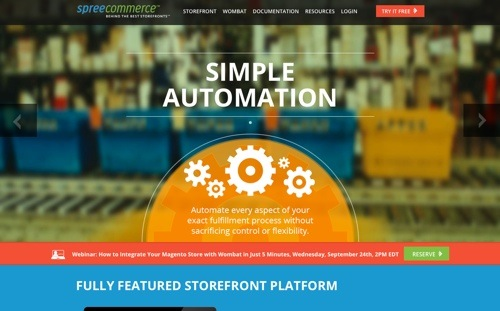
\includegraphics[width=0.5\textwidth]{figuras/cap1/SpreeCommerceWebsite.jpg}
		\caption{\nameSpreeCommerce \websiteINT \cite{online_SpreeCommerce}.}
	\end{figure}

	\item \textbf{\nameDrupalCommerce} es una aplicación \ecommerceCOM desarrollado por \commerceGuys. Construido sobre \drupalContManSys. \nameDrupalCommerce ofrece un sistema de administración de producto completo, carro de compra varios lenguajes y monedas; y forma de pago. La lista de extension de \nameDrupalCommerce es una integración completamente en\thirdParty para formas de pago,servicios de cumplimiento, aplicaciones de contabilidad, redes sociales y mucho mas. Paquetes de soporte técnico están disponibles por \commerceGuys.

	\begin{figure}[H]
		\centering
		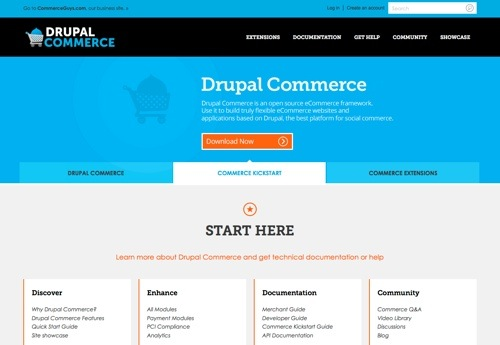
\includegraphics[width=0.5\textwidth]{figuras/cap1/DrupalCommerceWebsite.jpg}
		\caption{\nameDrupalCommerce \websiteINT \cite{online_DrupalCommerce}.}
	\end{figure}

	\item \textbf{\nameOsCommerce} (i.e., \openSourcePC \commerceCOM) es una de las primeras aplicaciones \ecommerceCOM \openSourcePC. Más de 7000 \freePC \addOns han sido subidos por su comunidad para customizar una \store \online. \nameOsCommerce es usado por cerca de 13000 sitios registrados. La comunidad de apoyo tiene aproximadamente 280000 miembros los cuales han contribuido con 1.5 millones de \posts en los foros. La comunidad directa junto con miembros de otra comunidad están disponibles en vivo en el \chat \room.

	\begin{figure}[H]
		\centering
		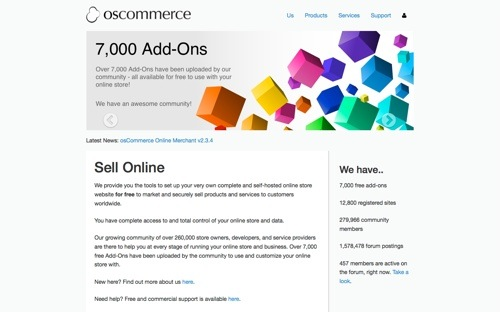
\includegraphics[width=0.5\textwidth]{figuras/cap1/osCommerceWebsite.jpg}
		\caption{\nameOsCommerce \websiteINT \cite{online_osCommerce}.}
	\end{figure}

	\item \textbf{\nameSimpleCart} es un \freePC y \openSourcePC \javaScriptNAME \shoppingCart. Con su pequeño tamaño, \nameSimpleCart está diseñado para mantener simple  y sitios con alto tráfico \runningCPT \fast. \nameSimpleCart tiene la habilidad de pagar con \paypalCheckout, \googleCheckout, y \amazonPayments. \email \checkoutCOM e integración con \AuthorizeNet llegarán pronto.
	
	\begin{figure}[H]
		\centering
		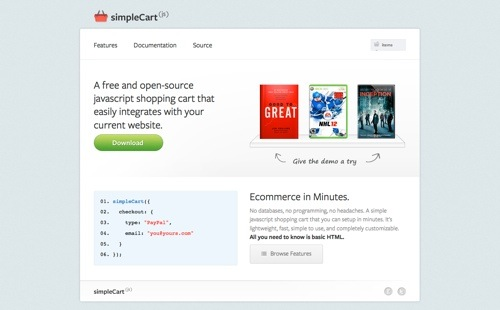
\includegraphics[width=0.5\textwidth]{figuras/cap1/simpleCartWebsite.jpg}
		\caption{\nameSimpleCart \websiteINT \cite{online_simpleCart}.}
	\end{figure}

	\item \textbf{\nameWooCommerce} es una aplicación \ecommerceCOM \freePC \openSourcePC que permite a los comerciantes transformar \wordPressNAME \sitesINT en \stores. \nameWooCommerce fue desarrollado por \wooThemes desde un \fork de \nameJigoshop. \nameWooCommerce tiene una larga variedad de  \pluginsAS y  \themesCPT de \wooThemes como de sitios \thirdParty, tales como \themeForest \cite{online_ThemeForest} y \codeCanyon \cite{online_CodeCanyon}. Con cerca de 4.5 millones de descargas desde \wordPressOrg\cite{online_WordPress}, \nameWooCommerce es una solución \ecommerceCOM muy popular para \wordPressNAME. Para obtener el soporte oficial de \wooThemes, es necesario comprar un producto. De otra manera, obtener ayuda desde la comunidad activa del foro.

	\begin{figure}[H]
		\centering
		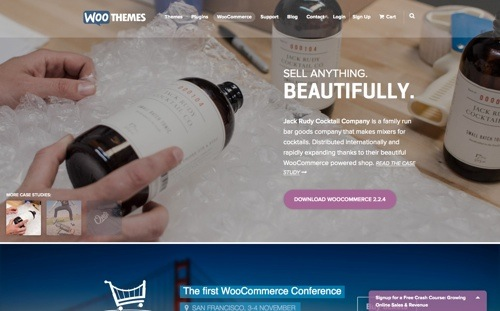
\includegraphics[width=0.5\textwidth]{figuras/cap1/WooCommerceWebsite.jpg}
		\caption{\nameWooCommerce \websiteINT \cite{online_WooCommerce}.}
	\end{figure}

	\item \textbf{\nameWPECommerce} es otra aplicación popular obtenida desde la conversión del  sitio \wordPressNAME a una \ecommerceCOM \store.\nameWPECommerce tiene cerca de 3 millones de descargas de \pluginAS desde \wordPressOrg\cite{online_WordPress}. Usa el propio \htmlNAME y \cssNAME y obtén el control completo sobre la vista y la experiencia de tu \online \store. \nameWPECommerce tiene una gran variedad de características estándar, incluyendo \multiTierPricing para descuentos por cantidad e integración con redes sociales para \marketing. Para soporte, hay tutoriales en vídeo y un foro en \wordPressOrg, también como consultantes de características para ayuda profesional.

	\begin{figure}[H]
		\centering
		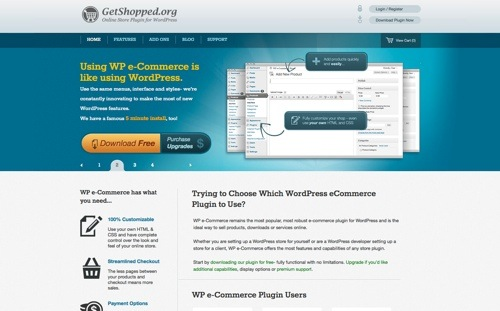
\includegraphics[width=0.5\textwidth]{figuras/cap1/WPECommerceWebsite.jpg}
		\caption{\nameWPECommerce \websiteINT \cite{online_WPECommerce}.}
	\end{figure}

	\item \textbf{\nameJigoshop} es una solución \ecommerceCOM \freePC y \openSourcePC basado en \wordPressNAME. Liberado en 2011, \nameJigoshop es el predecesor para \nameWooCommerce. \nameJigoshop tiene más de 30 \themesCPT, 100 extensiones y tres \theme \frameworksPC. \nameJigoshop es \freePC, así como el soporte a \wordPressOrg. Sin embargo, el acceso a la comunidad de \nameJigoshop comienza desde \$40 por mes.

	\begin{figure}[H]
		\centering
		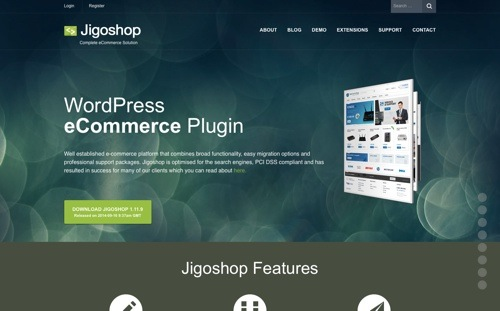
\includegraphics[width=0.5\textwidth]{figuras/cap1/JigoshopWebsite.jpg}
		\caption{\nameJigoshop \textit{website}\cite{online_Jigoshop}.}
	\end{figure}

\end{itemize}


%%%%%%%%%%%%%%%%%%%%%%%%%%%%%%%%%%%%%%%%%%%%%%%%%%%%%%%%%%%%%%%%%%%%%%%%%%%%%
%%%%%%%%%%%%%%%%  	RESUMEN GENERAL FRAMEWORKS ECOMMERCE 	 %%%%%%%%%%%%%%%%
%%%%%%%%%%%%%%%%%%%%%%%%%%%%%%%%%%%%%%%%%%%%%%%%%%%%%%%%%%%%%%%%%%%%%%%%%%%%%

%%%%%%%%%%%%%%%%%%%%%%%%%%%%%%%%%%%%%%%%%%%%%%%%%%%%%%%%%%%%%%%%%%%%%%%%%%%%%%
%%%%%%%%%%%%%%%%%%%		     RESUMEN GENERAL	   	%%%%%%%%%%%%%%%%%%%%%%%%%
%%%%%%%%%%%%%%%%%%%%%%%%%%%%%%%%%%%%%%%%%%%%%%%%%%%%%%%%%%%%%%%%%%%%%%%%%%%%%
\subsubsection{Resumen general de los \frameworksPC disponibles}

En \reftabla{tab:resume_technology_ecommerce} hay un resumen de información básica general sobre \shoppingCarts.
%Basic general information about the shopping carts including creator, software license and framework, and updates.

\begin{table}[H]
    \tiny
    \centering
%\begin{tabular}{ |C{0.3\paperwidth}|C{0.3\paperwidth}| }
\begin{tabular}{ |l|c|c|c|c|c| }

\hline
	&
	\freePC \dataBaseDB \backendAS support&
	Language&
	\wafAS&
	\License&
	version

\\ \hline
	\nameOpenCart &
	\mysqlNAME&
	\phpNAME&
	&
	\gplthreelicense &
	2.0.1.1
	
\\ \hline
	\namePrestaShop &
	\mysqlNAME&
	\phpNAME&
	&
	\opslicense &
	1.6.0.11
	
\\ \hline
	\nameMagento &
	\mysqlNAME&
	\phpNAME&
	\zendNAME \cite{online_zend_framework}&
	\opslicense &
	1.9.1.0
	
\\ \hline
	\nameZenCart &
	\mysqlNAME&
	\phpNAME&
	&
	\gpllicense &
	1.5.4
 
\\ \hline
	\nameSpreeCommerce &
	\mysqlNAME, \postgresql, \sqlitethree&
	\rubyNAME \cite{online_ruby_language}&
	\rubyonrailsNAME \cite{online_ruby_rails}&
	\bsdthreelicense&
	2.2.2

\\ \hline
	\nameDrupalCommerce &
	\mysqlNAME, \postgresql, \sqlitethree&
	\phpNAME&
	\drupalNAME \cite{online_drupal}&
	\gpllicense &
	1.10
	
\\ \hline
	\nameOsCommerce &
	\mysqlNAME&
	\phpNAME&
	&
	\gpllicense &
	2.3.4

\\ \hline
	\nameSimpleCart &
	&
	&
	&
	&
	
\\ \hline
	\nameWooCommerce &
	\mysqlNAME&
	\phpNAME&
	\wordPressNAME \cite{online_wordpress}&
	\gpllicense &
	2.2.7
	
\\ \hline
	\nameWPECommerce &
	&
	&
	&
	&
	
\\ \hline
	\nameJigoshop &
	\mysqlNAME&
	\phpNAME&
	\wordPressNAME \cite{online_wordpress}&
	\gpllicense &
	1.12.3
	
\\ \hline
\end{tabular}
    \caption{ Resumen general de los \frameworksPC disponibles}
    \label{tab:resume_technology_ecommerce}
\end{table}



%
%\begin{table}[h!]
%    \tiny
%    \centering
%%\begin{tabular}{ |C{0.3\paperwidth}|C{0.3\paperwidth}| }
%\begin{tabular}{ |l|c|c|c|c|c|c| }
%\hline
%	&
%	traider\cite{online_Traider}&
%	ReactionCommerce\cite{online_reactionCommerce}&
%	NodeShop\cite{online_NodeShop}&
%	Forward\cite{online_Forward}&
%	Ottemo \cite{online_framework_ottemo_officialsite}&
%	ZRECommerce \cite{online_framework_zrecommerce_officialsite}
% 
%\\ \hline
%	Tecnología &
%	bootstrap, nodejs and mongodb &
%	Nodejs, Meteor, Mongodb, CoffeScript, Bootstrap, Docker&
%	&
%	
%
%\\ \hline
%	Mobile &
%	&
%	&
%	&
%\\ \hline
%	version &
%	&
%	&
%	0.06 ( 21/08/2013 )&
%	0.1
%
%\\ \hline
%\end{tabular}
%    \caption{ Resumen tecnologías entre diferentes opciones \textit{e-Commerce}}
%    \label{tab:resume_technology_ecommerce2}
%\end{table}


%%%%%%%%%%%%%%%%%%%%%%%%%%%%%%%%%%%%%%%%%%%%%%%%%%%%%%%%%%%%%%%%%%%%%%%%%%%%%
%%%%%%%%%%%%%%%%%%%		  CUSTOMERS FEATURES		%%%%%%%%%%%%%%%%%%%%%%%%%
%%%%%%%%%%%%%%%%%%%%%%%%%%%%%%%%%%%%%%%%%%%%%%%%%%%%%%%%%%%%%%%%%%%%%%%%%%%%%

\begin{table}[H]
    \tiny
    \centering
%\begin{tabular}{ |C{0.3\paperwidth}|C{0.3\paperwidth}| }
\begin{tabular}{ |l|c|c|c|c|c|c|c| }

\hline
	&
	Buscar&
	Imagen \itemCOM&
	\raiting \itemCOM&
	\review \itemCOM&
	\wishlist&
	\itemsCOM populares&
	Redes sociales

\\ \hline
	\nameOpenCart &
	&
	&
	&
	&
	&
	&
	
\\ \hline
	\namePrestaShop &
	\anwerYes&
	\anwerYes&
	\anwerYes&
	\anwerYes&
	\anwerYes&
	\anwerYes&
	\anwerYes
	
\\ \hline
	\nameMagento &
	\anwerYes&
	\anwerYes&
	\anwerYes&
	\anwerYes&
	\anwerYes&
	\anwerYes&
	\anwerYes
	
\\ \hline
	\nameZenCart &
	\anwerYes&
	\anwerYes&
	\anwerYes&
	\anwerYes&
	\freePC \addOn&
	\anwerYes&
	\freePC \addOn
 
\\ \hline
	\nameSpreeCommerce &
	&
	&
	&
	&
	&
	&

\\ \hline
	\nameDrupalCommerce &
	\anwerYes&
	\anwerYes&
	\anwerYes&
	\anwerYes&
	\anwerYes&
	\anwerYes&
	\anwerYes
	
\\ \hline
	\nameOsCommerce &
	\anwerYes&
	\anwerNo&
	\anwerYes&
	\anwerYes&
	\anwerNo&
	\anwerYes&
	\anwerYes

\\ \hline
	\nameSimpleCart &
	&
	&
	&
	&
	&
	&
	
\\ \hline
	\nameWooCommerce &
	&
	&
	&
	&
	&
	&
	
\\ \hline
	\nameWPECommerce &
	&
	&
	&
	&
	&
	&
	
\\ \hline
	\nameJigoshop &
	\anwerYes&
	\anwerYes&
	\anwerYes&
	\anwerYes&
	\anwerYes&
	\anwerYes&
	\anwerYes
	
\\ \hline
\end{tabular}
    \caption{ Características de \customers}
    \label{tab:customers_features_ecommerce}
\end{table}

%%%%%%%%%%%%%%%%%%%%%%%%%%%%%%%%%%%%%%%%%%%%%%%%%%%%%%%%%%%%%%%%%%%%%%%%%%%%%
%%%%%%%%%%%%%%%%%%%	  ADMINISTRATION AREA FEATURES	%%%%%%%%%%%%%%%%%%%%%%%%%
%%%%%%%%%%%%%%%%%%%%%%%%%%%%%%%%%%%%%%%%%%%%%%%%%%%%%%%%%%%%%%%%%%%%%%%%%%%%%

\subsubsection{Características de administración}

Información sobre las características que los \shoppingCarts ofrecen.

\begin{table}[h!]
    \tiny
	\centering
%\begin{tabular}{ |C{0.3\paperwidth}|C{0.3\paperwidth}| }
\begin{tabular}{ |l|c|c|c| }	

\hline
	&
	Estadísticas &
	Control de \stock &
	Editor \wysiwyg

\\ \hline
	\nameOpenCart &
	&
	&
	
\\ \hline
	\namePrestaShop &
	\anwerYes&
	\anwerYes&
	\anwerYes
	
\\ \hline
	\nameMagento&
	\anwerYes&
	\anwerYes&
	\anwerYes
	
\\ \hline
	\nameZenCart &
	\anwerYes&
	\anwerYes&
	\freePC \addOn
 
\\ \hline
	\nameSpreeCommerce &
	&
	&
	

\\ \hline
	\nameDrupalCommerce&
	\anwerYes&
	\anwerYes&
	\anwerYes
	
\\ \hline
	\nameOsCommerce &
	\anwerYes&
	\anwerYes&
	\freePC \addOn

\\ \hline
	\nameSimpleCart &
	&
	&
	
	
\\ \hline
	\nameWooCommerce &
	&
	&
	
	
\\ \hline
	\nameWPECommerce &
	&
	&
	
	
\\ \hline
	\nameJigoshop &
	\anwerYes&
	\anwerYes&
	\anwerYes
	
\\ \hline

\end{tabular}
    \caption{ Soporte de \checkoutCOM }
    \label{tab:administration_area_features}
\end{table}


%%%%%%%%%%%%%%%%%%%%%%%%%%%%%%%%%%%%%%%%%%%%%%%%%%%%%%%%%%%%%%%%%%%%%%%%%%%%%
%%%%%%%%%%%%%%%%%%%	  ADMINISTRATION AREA FEATURES	%%%%%%%%%%%%%%%%%%%%%%%%%
%%%%%%%%%%%%%%%%%%%%%%%%%%%%%%%%%%%%%%%%%%%%%%%%%%%%%%%%%%%%%%%%%%%%%%%%%%%%%

\subsubsection{Características de \rewards para \customers}

Información sobre las características que los \shoppingCarts ofrecen.

\begin{table}[h!]
    \tiny
	\centering
%\begin{tabular}{ |C{0.3\paperwidth}|C{0.3\paperwidth}| }
\begin{tabular}{ |l|c|c|c|c|c|c|c| }	

\hline
	&
	Cupones&
	Certificados de \gifts&
	Descuentos \membership&
	Categorías \membershipOnly&
	\itemCOM \membershipOnly&
	Puntos de \reward&
	Ofertas especiales

\\ \hline
	\nameOpenCart &
	&
	&
	&
	&
	&
	&
	
\\ \hline
	\namePrestaShop &
	\anwerYes&
	\anwerYes&
	\anwerYes&
	\anwerYes&
	\anwerYes&
	\anwerYes
	
\\ \hline
	\nameMagento&
	\anwerYes&
	\anwerYes&
	\anwerYes&
	\anwerYes&
	\thirdPartyModule&
	\anwerYes
	
\\ \hline
	\nameZenCart &
	\anwerYes&
	\anwerYes&
	\anwerYes&
	\anwerNo&
	\anwerNo&
	\anwerYes&
	\anwerYes
 
\\ \hline
	\nameSpreeCommerce &
	&
	&
	&
	&
	&
	&
	

\\ \hline
	\nameDrupalCommerce&
	\anwerYes&
	\anwerYes&
	\anwerYes&
	\anwerYes&
	\anwerYes&
	\anwerNo&
	\anwerYes
	
\\ \hline
	\nameOsCommerce &
	\anwerYes&
	\anwerYes&
	\freePC \addOn&
	&
	&

\\ \hline
	\nameSimpleCart &
	&
	&
	&
	&
	&
	&
	
	
\\ \hline
	\nameWooCommerce &
	&
	&
	&
	&
	&
	&
	
	
\\ \hline
	\nameWPECommerce &
	&
	&
	&
	&
	&
	&
	
\\ \hline
	\nameJigoshop &
	\anwerYes&
	\anwerYes&
	\anwerYes&
	\anwerYes&
	\anwerYes&
	\anwerYes&
	\anwerYes
	
\\ \hline

\end{tabular}
    \caption{ Características de \rewards para \customers }
    \label{tab:customer_reward_features}
\end{table}


%%%%%%%%%%%%%%%%%%%%%%%%%%%%%%%%%%%%%%%%%%%%%%%%%%%%%%%%%%%%%%%%%%%%%%%%%%%%%
%%%%%%%%%%%%%%%%%%%%%%%%%%%%  CHECKOUT SUPPORT  %%%%%%%%%%%%%%%%%%%%%%%%%%%%%
%%%%%%%%%%%%%%%%%%%%%%%%%%%%%%%%%%%%%%%%%%%%%%%%%%%%%%%%%%%%%%%%%%%%%%%%%%%%%

\subsubsection{Soporte de \checkoutCOM}

En \reftabla{tab:checkout_support} se encuentra disponible la información  sobre los \checkoutCOM disponibles.

\begin{table}[h!]
    \tiny
	\centering
%\begin{tabular}{ |C{0.3\paperwidth}|C{0.3\paperwidth}| }
\begin{tabular}{ |l|c|c|c| }	

\hline
	&
	\googleCheckout &
	\paypalCheckout &
	\amazonCheckout

\\ \hline
	\nameOpenCart &
	&
	&
	
\\ \hline
	\namePrestaShop &
	\anwerYes&
	\anwerYes&
	\anwerYes
	
\\ \hline
	\nameMagento&
	\anwerYes&
	\anwerYes&
	\freePC \addOn
	
\\ \hline
	\nameZenCart &
	\freePC \addOn&
	\anwerYes&
	\answerunknown
 
\\ \hline
	\nameSpreeCommerce &
	&
	&
	

\\ \hline
	\nameDrupalCommerce&
	\anwerYes&
	\anwerYes&
	\answerunknown
	
\\ \hline
	\nameOsCommerce &
	\anwerNo&
	\anwerNo&
	\answerunknown

\\ \hline
	\nameSimpleCart &
	&
	&
	
	
\\ \hline
	\nameWooCommerce &
	&
	&
	
	
\\ \hline
	\nameWPECommerce &
	&
	&
	
	
\\ \hline
	\nameJigoshop &
	\anwerYes&
	\anwerYes&
	\anwerYes
	
\\ \hline

\end{tabular}
    \caption{ Soporte de \checkoutCOM }
    \label{tab:checkout_support}
\end{table}


%%%%%%%%%%%%%%%%%%%%%%%%%%%%%%%%%%%%%%%%%%%%%%%%%%%%%%%%%%%%%%%%%%%%%%%%%%%%%%%
%%%%%%%%%%%%%%%%%%%	 	REAL TIME SHIPPING CALCULATION 		%%%%%%%%%%%%%%%%%%%
%%%%%%%%%%%%%%%%%%%%%%%%%%%%%%%%%%%%%%%%%%%%%%%%%%%%%%%%%%%%%%%%%%%%%%%%%%%%%%%

\subsubsection{Cálculo \shipping \realTimeINT}

Información sobre si \shoppingCarts tienen como característica cálculo \shipping \realTimeINT permite calcular cuanto tiempo costará enviar una orden in \realTimeINT cuando el cliente \checkoutCOM una orden.
%Information about if the Shopping Carts have Real Time Shipping Calculation built in to be able to calculate how much it will cost to ship an order in real time when the customer checks out an order.
\begin{table}[H]
    \tiny
   \centering
%\begin{tabular}{ |C{0.3\paperwidth}|C{0.3\paperwidth}| }
\begin{tabular}{ |l|c|c|c| }

\hline
	&
	\dhlName &
	\fedExName &
	\upsName

\\ \hline
	\nameOpenCart &
	&
	&
	
	
\\ \hline
	\namePrestaShop &
	\anwerNo&
	\anwerYes&
	\anwerYes
	
\\ \hline
	\nameMagento&
	\anwerYes&
	\anwerYes&
	\anwerYes
	
\\ \hline
	\nameZenCart &
	\freePC \addOn&
	\freePC \addOn&
	\anwerYes
 
\\ \hline
	\nameSpreeCommerce &
	&
	&

\\ \hline
	\nameDrupalCommerce&
	&
	&
	
\\ \hline
	\nameOsCommerce &
	\anwerNo&
	\anwerNo&
	\anwerNo

\\ \hline
	\nameSimpleCart &
	&
	&
	
\\ \hline
	\nameWooCommerce &
	&
	&
	
\\ \hline
	\nameWPECommerce &
	&
	&
	
\\ \hline
	\nameJigoshop &
	\anwerYes&
	\anwerYes&
	\anwerYes
	
\\ \hline

\end{tabular}
    \caption{Cálculo \shipping \realTimeINT}
    \label{tab:general_features_ecommerce}
\end{table}


%%%%%%%%%%%%%%%%%%%%%%%%%%%%%%%%%%%%%%%%%%%%%%%%%%%%%%%%%%%%%%%%%%%%%%%%%%%%%%%
%%%%%%%%%%%%%%%%%%%	  	Shipment tracking integration 		%%%%%%%%%%%%%%%%%%%
%%%%%%%%%%%%%%%%%%%%%%%%%%%%%%%%%%%%%%%%%%%%%%%%%%%%%%%%%%%%%%%%%%%%%%%%%%%%%%%

\subsubsection{Integración \tracking \shipping}

Información sobre si \shoppingCarts tienen integración de \tracking \shipping para mostrar a los \customers información de \tracking en la página de ordenes.
%Information about if the Shopping Carts have Shipment Tracking Integration to show the customers the tracking information on the View Order pages.
\begin{table}[H]
    \tiny
	\centering
%\begin{tabular}{ |C{0.3\paperwidth}|C{0.3\paperwidth}| }
\begin{tabular}{ |l|c|c|c| }

\hline
	&
	\dhlName &
	\fedExName &
	\upsName

\\ \hline
	\nameOpenCart &
	&
	&
	
\\ \hline	
	\namePrestaShop &
	\anwerNo&
	\anwerYes&
	\anwerYes
	
\\ \hline
	\nameMagento&
	\anwerYes&
	\anwerYes&
	\anwerYes
	
\\ \hline
	\nameZenCart &
	\freePC \addOn&
	\freePC \addOn&
	\freePC \addOn
 
\\ \hline
	\nameSpreeCommerce &
	&
	&

\\ \hline
	\nameDrupalCommerce&
	&
	&
	
\\ \hline
	\nameOsCommerce &
	\anwerNo&
	\anwerNo&
	\anwerNo

\\ \hline
	\nameSimpleCart &
	&
	&
	
\\ \hline
	\nameWooCommerce &
	&
	&
	
\\ \hline
	\nameWPECommerce &
	&
	&
	
\\ \hline
	\nameJigoshop &
	\anwerYes&
	\anwerYes&
	\anwerYes
	
\\ \hline
\end{tabular}
    \caption{Integración \tracking \shipping}
    \label{tab:Shipment_tracking_integration}
\end{table}


%%%%%%%%%%%%%%%%%%%%%%%%%%%%%%%%%%%%%%%%%%%%%%%%%%%%%%%%%%%%%%%%%%%%%%%%%%%%%